\chapter{Efficient Retrieval}

\begin{multicols*}{2}
\section{Dimension Reduction}

\noindent To reduce sparsity problem, we use dimensionality reduction technique, such as truncated singular value decomposition, to discard some small / unimportant singular values. 

\section{Efficient Cosine Ranking}
\noindent To compute $K$ highest-scoring document for a query, we need to compute cosine similarity for all documents. To improve efficiency, we can consider only $K$ documents that likely to be among $K$ highest scoring documents. 

\subsection{Index Elimination}
\noindent Rule 1: only consider documents that contain at least one query term \\
\noindent Rule 2: only consider high-IDF query terms. Low-IDF terms are likely to be stopwords and contribute little to the scores. \\
\noindent Rule 3: only consider documents that contain many query terms. This can be done during posting traversal. 

\subsection{Champion Lists}
\noindent Precompute, for each term $t$ in the dictionary, the set of the $r$ documents with the highest weights for $t$; the value of $r$ is chosen in advance. We call this set of $r$ documents the champion list for term $t$.\\

\noindent At query time, we only compute scores for documents in the champion list for some query terms. 

\subsection{Static Quality Scores}
\noindent We want top-ranking documents to be both relevant and authoritative. Let the query-independent quality score as $g(d)$, the net score:
$$\text{netscore}(\vec{q},\vec{d})=g(d) + \text{cosine} (\vec{q},\vec{d})$$

\noindent We get the top $K$ documents by net score

\subsection{High and Low Lists}
\noindent We maintain two posting lists called high and low. We first traverse high lists first to get top $K$ documents. If we do not get enough document, then only we traverse low lists. 

\subsection{Cluster Pruning}
\noindent We first pick $\sqrt{N}$ documents at random (leaders), then pre-compute the nearest leader for all documents. \\
\noindent We process query by finding its nearest leader $L$ and find $K$ nearest document from $L$’s followers

\section{Parametric and Zone Indexes}
\noindent There could be some metadata / fields for each documents. We want to search by fields. \\

\noindent A zone is a region of documents that can contain an arbitrary amount of text. We build inverted indexes on zones to permit querying.

\begin{center}
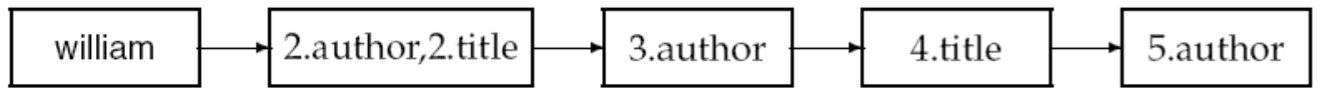
\includegraphics[width=8cm]{zone-index}
\end{center}

\section{Tiered Indexes}
\noindent Break postings up into a hierarchy of lists. Inverted index thus broken up into tiers of decreasing importance.\\

\noindent We process query by using top tier unless it fails to yield $K$ documents. 

\section{Aggregate Scores}

$$\text{score} = \alpha \times \text{cosine}(\vec{q},\vec{d}) + \beta \times g(d) + \gamma \times \text{proximity}(\vec{q},\vec{d})$$

\end{multicols*}
